\documentclass[fullscreen=true, bookmarks=true, hyperref={pdfencoding=unicode}]{beamer}
\usepackage[utf8]{inputenc}                                % Кодировка
\usepackage[english,russian]{babel}                        % Переносы
\usepackage{xcolor}                                        % Работа с цветом
\usepackage{amsmath,amssymb,amsfonts}                      % Символы АМО
\usepackage{graphicx}                                      % Графика
\usepackage[labelsep=period]{caption}                      % Разделитель в подписях к рисункам и таблицам
\usepackage{hhline}                                        % Для верстки линий в таблицах
\usepackage{tikz}                                          % Для простых рисунков в документе
\usepackage{fancybox}                                      % Пакет для отрисовки рамок
\usepackage{verbatim}                                      % Для вставки кода в презентацию
\usepackage{animate}                                       % Для вставки видео в презентацию
\usepackage{xmpmulti}                                      % Для вставки gif в презентацию
\usepackage{multirow}

\usetikzlibrary{arrows,snakes,backgrounds}                 % Для отрисовки стрелок

\graphicspath{{images/}}                                   % Путь до рисунков
\setbeamertemplate{caption}[numbered]                      % Включение нумерации рисунков

\definecolor{links}{HTML}{2A1B81}                          % blue for url links
\hypersetup{colorlinks,linkcolor=,urlcolor=links}          % nothing for others

\usetheme{boxes}
\usecolortheme{crane}

\usepackage{pythonhighlight}

\newtheorem*{question}{Вопрос}

\title{Лекция 2. Свёрточные нейронные сети, продолжение}
\author{Александр Юрьевич Авдюшенко}
\institute{МКН СПбГУ}
\date{24 февраля 2022}
\titlegraphic{
\includegraphics[keepaspectratio,width=0.5\textwidth]{logo_fmkn.png}}

\begin{document}
%\unitlength=2mm

% выводим заглавие
\begin{frame}
\transdissolve[duration=0.2]
\titlepage
\end{frame}

\begin{frame}
  \frametitle{Пятиминутка}
  \begin{itemize}
    \item Определите операцию свёртки для нейронных сетей
    \item Выпишите основные особенности сети AlexNet
    \item Выпишите несколько популярных функций активации
  \end{itemize}
\end{frame}


\begin{frame}
  \frametitle{Развитие свёрточных сетей}
  \framesubtitle{или краткая история ImageNet}
  \begin{center}
    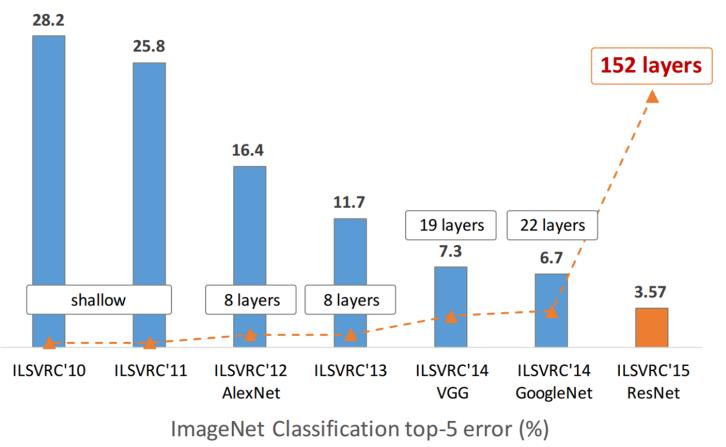
\includegraphics[keepaspectratio,
                     width=0.7\paperwidth]{image-net-history.jpg}
  \end{center}
\end{frame}


\begin{frame}
  \frametitle{AlexNet (Krizhevsky, Sutskever, Hinton, 2012)}
  \framesubtitle{Победитель конкурса ImageNet того времени}
  \begin{center}
    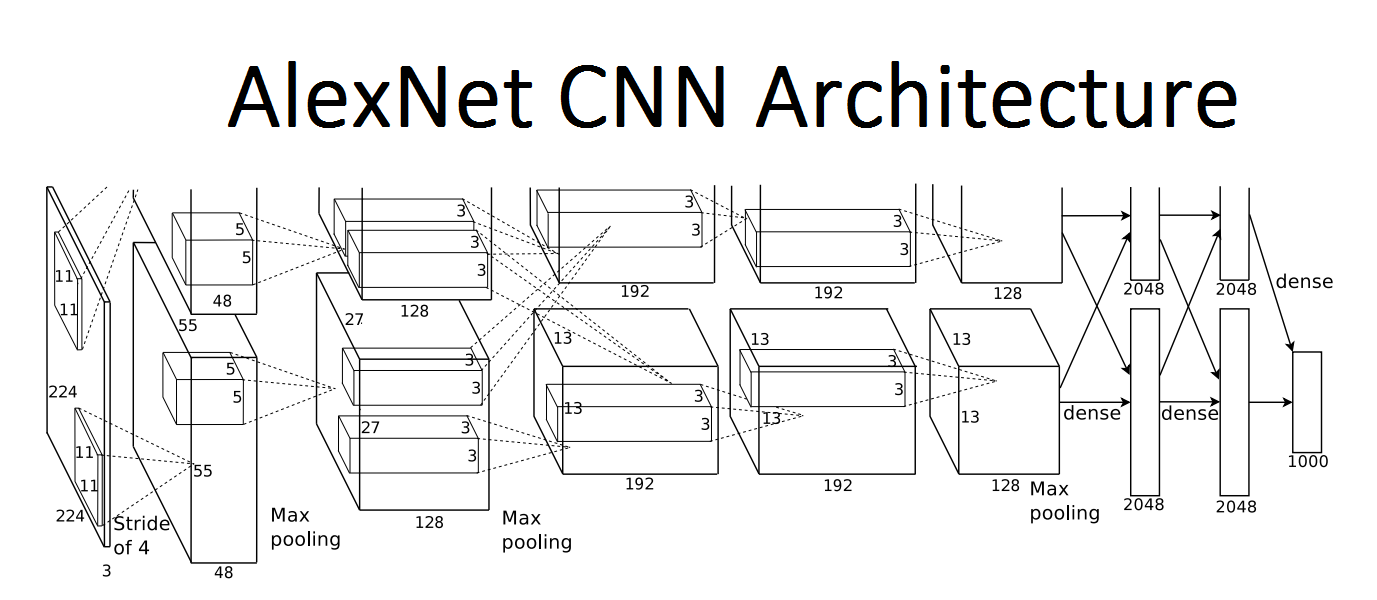
\includegraphics[keepaspectratio,
                     width=0.5\paperwidth]{AlexNetCNN.png}
  \end{center}
  \begin{itemize}
    \item ReLU
    \item аугментация данных
    \item {\it dropout 0.5}
    \item {\it batch normalization} (размер батча 128)
    \item SGD Momentum 0.9
    \item L2 регуляризация 5e-4
    \item Learning rate 1e-2, потом уменьшение в 10 раз после стабилизации качества на тесте
  \end{itemize}

    Финальное качество top5 на ImageNet — 25.8\% ->16.4\%
\end{frame}


{ % all template changes are local to this group.
    \setbeamertemplate{navigation symbols}{}
    \begin{frame}<article:0>[plain]
        \begin{tikzpicture}[remember picture,overlay]
            \node[at=(current page.center)] {
                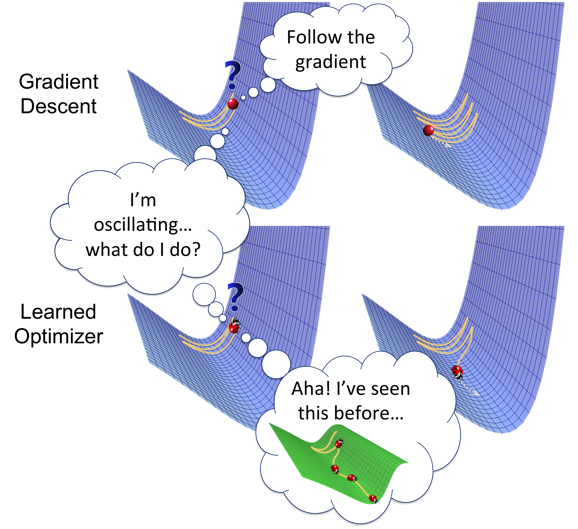
\includegraphics[keepaspectratio,
                                 width=\paperwidth,
                                 height=\paperheight]{optimization_mem.png}
            };
        \end{tikzpicture}
     \end{frame}
}

\begin{frame}
  \frametitle{Методы оптимизации нейронных сетей}
  {\bf AdaGrad}
  \begin{align*}
     G &= G + \mathcal{L}_i^\prime(w) \odot \mathcal{L}_i^\prime(w) \\
     w &= w - {\eta_t} {\mathcal{L}_i^\prime(w)}\oslash{\sqrt{G + \varepsilon}}
  \end{align*}

  $\eta_t$ может быть зафиксирован, к примеру $\eta_t = 0.01$,

  $\odot, \oslash$ — покомпонентное умножение и деление векторов

  Преимущества:
  \begin{itemize}
    \item $\mathcal{L}_i^\prime(w)$ — градиент на $i$-ом объекте
    \item отдельная адаптация шага для каждого измерения
    \item подходит для разреженных данных
  \end{itemize}

 Недостаток:
 \begin{itemize}
   \item $G$ постоянно увеличивается, что может привести к остановке обучения
 \end{itemize}
\end{frame}


\begin{frame}
  {RMSProp (running mean square)}

  Выравнивание скоростей изменения весов скользящим средним
  \begin{align*}
     G &= \color{red}{\alpha} G + \color{red}{(1 - \alpha)}\mathcal{L}_i^\prime(w) \odot \mathcal{L}_i^\prime(w) \\
     w &= w - {\eta_t} {\mathcal{L}_i^\prime(w)}\oslash{\sqrt{G + \varepsilon}}
  \end{align*}

  $\eta_t$ может быть зафиксирован, к примеру $\eta_t = 0.01$

  Преимущества:
  \begin{itemize}
    \item те же, что и у AdaGrad
    \item $G$ не растёт бесконтрольно
  \end{itemize}

 Недостатки:
 \begin{itemize}
   \item в самом начале обучения $G$ усредняется по нулевым предыдущим значениям
   \item нет учёта моментов
 \end{itemize}
\end{frame}


\begin{frame}[t]
  \frametitle{Adam (adaptive momentum)}

  \begin{align*}
  \nu &= \gamma \nu + (1-\gamma) \mathcal{L}_i^\prime(w) \quad     &\hat\nu = \nu(1-\gamma^k)^{-1} \\
    G &= {\alpha} G + {(1 - \alpha)}\mathcal{L}_i^\prime(w) \odot \mathcal{L}_i^\prime(w) \quad &\hat G = G(1-\alpha^k)^{-1} \\
    w &= w - {\eta_t}\hat\nu \oslash (\sqrt{\hat G + \varepsilon})
  \end{align*}

  $k$ — номер итерации, $\gamma = 0.9, \alpha = 0.999, \varepsilon = 10^{-8}$

   Преимущества:
   \begin{itemize}
     \item те же, что и у RMSProp
     \item калибровка $\hat\nu, \hat G$ увеличивает $\nu, G$ на первых итерациях
     \item есть учёт моментов
   \end{itemize}
\end{frame}


\begin{frame}[t]
  \frametitle{Nadam (Nesterov-accelerated adaptive momentum)}

  Те же формулы для $\nu, \hat\nu, G, \hat G$

  $ w = w - {\eta_t}\color{red}{\left(\gamma\hat\nu + \frac{1-\gamma}{1-\gamma^k}\mathcal{L}_i^\prime(w) \right)} \oslash (\sqrt{\hat G + \varepsilon})
  $

  $k$ — номер итерации, $\gamma = 0.9, \alpha = 0.999, \varepsilon = 10^{-8}$

  \noindent\rule{8cm}{0.4pt}

  {\it T. Dozat}. Incorporating Nesterov Momentum into Adam. ICLR-2016
\end{frame}


\begin{frame}
  \frametitle{Пример сходимости}
  \begin{center}
    \animategraphics[loop,width=0.5\paperwidth,autoplay]{8}{gd_animation-}{0}{118}
  \end{center}

  \noindent\rule{8cm}{0.4pt}

   Источник: \href{http://www.denizyuret.com/2015/03/alec-radfords-animations-for.html}{http://www.denizyuret.com/2015/03/alec-radfords-animations-for.html}
\end{frame}


\begin{frame}
    \begin{question}
    Какой метод и как выбрать?
    \end{question}
\end{frame}


\begin{frame}
  \frametitle{Диагональный метод Левенберга-Марквaрдта}
  \framesubtitle{напоминание}
  Метод Ньютона-Рафсона (второго порядка):

  $$ w = w - \eta(\mathcal{L}^{\prime\prime}_i(w))^{-1} \mathcal{L}^{\prime}_i(w),$$

  где $\mathcal{L}^{\prime\prime}_i(w) = \frac{\partial^2 \mathcal{L}_i(w)}{\partial w_{jh} \partial w_{j^\prime h^\prime}}$ — гессиан

  {\bf Эвристика}. Считаем, что гессиан диагонален:

    $w_{jh} = w_{jh} - \eta \left(\frac{\partial^2 \mathcal{L}_i(w)}{\partial w^2_{jh}} + \mu \right)^{-1} \frac{\partial \mathcal{L}_i(w)}{\partial w_{jh}}$,

    $\eta$ — темп обучения, можно полагать $\eta = 1$

    $\mu$ — параметр, предотвращающий обнуление знаменателя

    Отношение $\eta/\mu$ есть темп обучения на ровных участках функционала $\mathcal{L}_i(w)$, где вторая производная обнуляется.
\end{frame}


\begin{frame}
  \frametitle{Взрыв градиента (gradient exploding)}
  \begin{center}
    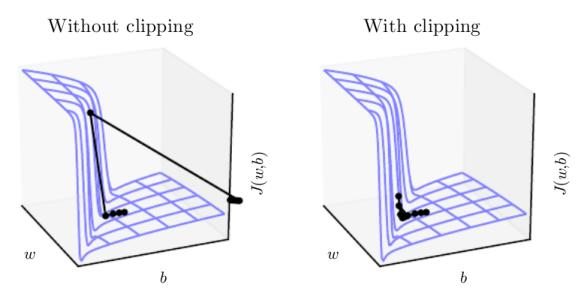
\includegraphics[keepaspectratio,
                     width=0.6\paperwidth]{gradient_exploding.jpg}
  \end{center}
  Можно отсекать (\pyth{np.clip}) по значениям или по модулю значений.

  \noindent\rule{8cm}{0.4pt}

  Источник: \href{https://neptune.ai/blog/understanding-gradient-clipping-and-how-it-can-fix-exploding-gradients-problem}{https://neptune.ai/blog/understanding-gradient-clipping-and-how-it-can-fix-exploding-gradients-problem}
\end{frame}


\begin{frame}
  \frametitle{Методы регуляризации}

  {\bf Dropout — метод случайных отключений нейронов}

  {\bf Этап обучения}: делая градиентный шаг $\mathcal{L}_i(w) \to \min\limits_w$, отключаем $h$-ый нейрон $\ell$-го слоя с вероятностью $p_\ell$:

  $x_{ih}^{\ell + 1} = \color{red}{\xi_h^\ell} \sigma_h (\sum\limits_j w_{jh} x_{ij}^\ell), \ \ \
   \color{red}{P(\xi_h^\ell = 0) = p_\ell}$

  {\bf Этап применения}: включаем все нейроны, но с поправкой:

  $x_{ih}^{\ell + 1} = \color{red}{(1 - p_\ell)} \sigma_h(\sum\limits_j w_{jh} x_{ij}^\ell)$

  \begin{center}
    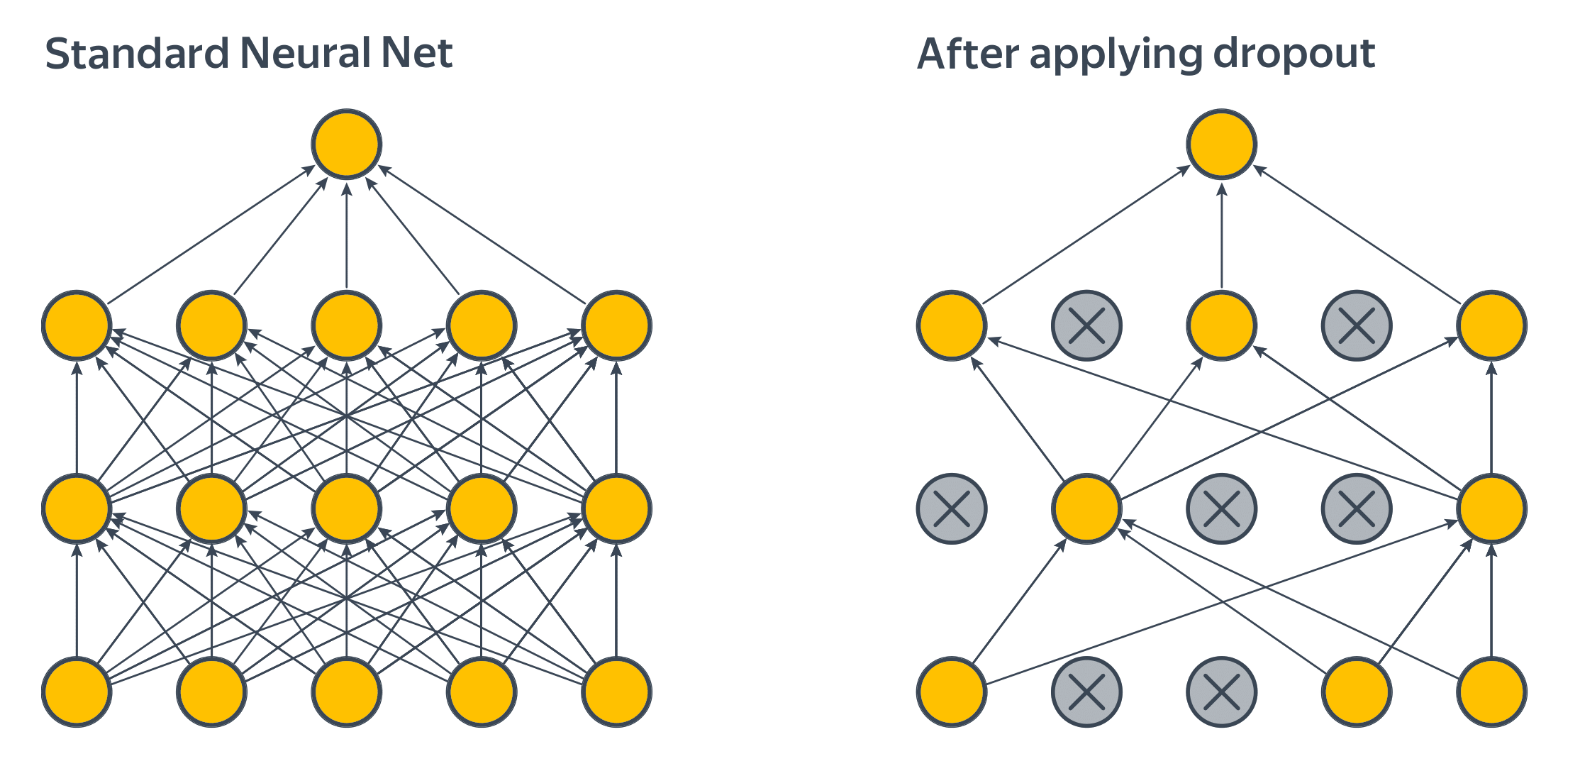
\includegraphics[keepaspectratio,
                     width=.6\paperwidth]{dropout_shad.png}
  \end{center}
\end{frame}


\begin{frame}
    \begin{question}
    Какая особенность появляется при таком применении?
    \end{question}
\end{frame}


\begin{frame}
  \frametitle{Inverted Dropout}

  На практике чаще используют не Dropout, а Inverted Dropout

  {\bf Этап обучения}:

  $x_{ih}^{\ell + 1} = \color{red}{\frac{1}{1-p_\ell} \xi_h^\ell} \sigma_h (\sum\limits_j w_{jh} x_{ij}^\ell), \ \ \
   P(\xi_h^\ell = 0) = p_\ell$

  {\bf Этап применения} не требует ни модификаций, ни знания $p_\ell$:

  $x_{ih}^{\ell + 1} = \sigma_h(\sum\limits_j w_{jh} x_{ij}^\ell)$

  $L_2$-регуляризация предотвращает рост параметров на обучении:

  $\mathcal{L}_i(w) + \frac{\lambda}{2} \|w\|^2 \to \min\limits_w$

  Градиентный шаг с Dropout и $L_2$-регуляризацией:

  $w = w (1 - \eta \lambda) - \eta\color{red}{\frac{1}{1-p_\ell} \xi_h^\ell} \mathcal{L}_i^\prime(w)$
\end{frame}


\begin{frame}
  \frametitle{Интерпретации Dropout}

  \begin{itemize}
    \item аппроксимируем простое голосование по $2^N$ сетям с общим набором $N$ нейронов
    \item регуляризация: выбираем из всех сетей более устойчивую к утрате $pN$ нейронов, моделируя надёжность мозга
    \item уменьшаем переобучение, заставляя разные части сети решать одну и ту же исходную задачу
  \end{itemize}

  \begin{center}
    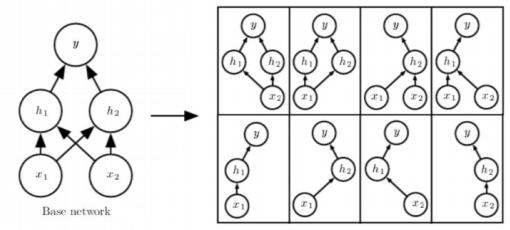
\includegraphics[keepaspectratio,
                     width=0.6\paperwidth]{dropout_interpretation.jpg}
  \end{center}
\end{frame}


\begin{frame}
  \frametitle{Batch normalization (пакетная нормализация данных)}

  $B = \{ x_i\}$ — пакеты (mini-batch) данных

  Усреднение градиентов $\mathcal{L}_i(w)$ по пакету ускоряет сходимость.

  $B^\ell = \{ u_i^\ell\}$ — векторы объектов $x_i$ на выходе $\ell$-го слоя

  1. Нормировать каждую $j$-ю компоненту вектора $u_i^\ell$ по пакету

  $$
    \hat u_{ij}^\ell = \frac{u_{ij}^\ell - \mu_j}{\sqrt{\sigma_j^2 + \varepsilon}}; \quad
    \mu_j = \frac{1}{|B|} \sum\limits_{x_i \in B} u_{ij}^\ell; \quad
    \sigma_j^2 = \frac{1}{|B|} \sum\limits_{x_i \in B} (u_{ij}^\ell - \mu_j)^2
  $$

  2. Добавить линейный слой с настраивыми весами:

  $$ \tilde u_{ij}^\ell = \gamma_j^\ell \hat u_{ij}^\ell + \beta_j^\ell $$

  3. Параметры $\gamma_j^\ell, \beta_j^\ell$ настраиваются BackProp
\end{frame}


\begin{frame}
  \frametitle{Начальное приближение весов}
  \begin{center}
    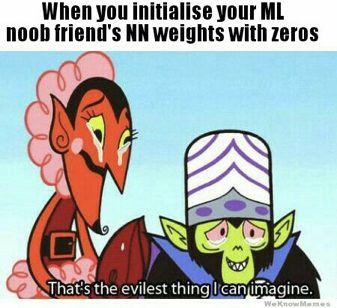
\includegraphics[keepaspectratio,
                     width=.4\paperwidth]{weight_init_meme.jpg}
  \end{center}
\end{frame}


\begin{frame}
    \frametitle{Следим за изменениями дисперсий}
    \framesubtitle{как значений нейронов, так и градиентов при обратном распространении}
  Выравнивание дисперсий и нейронов, и градиентов в разных слоях — инициализация Ксавье для $\tanh$:

  $$ w_j \sim U \left[ -\frac{{6}}{\sqrt{n_{in}+n_{out}}}, \frac{{6}}{\sqrt{n_{in}+n_{out}}} \right]$$

  $n_{in},\ n_{out}$ — количество нейронов в предыдущем и текущем слоях соотвественно

  Вывод и подробности есть \href{https://ml-handbook.ru/chapters/neural_nets/training}{в учебнике ШАД}.
  \pause
  \begin{question}
  Что делать в случае активации ReLU?
  \end{question}
\end{frame}


\begin{frame}
  \frametitle{Другие способы инициализации}
  \begin{enumerate}
    \item Послойное обучение нейронов, как линейных моделей
      \begin{itemize}
        \item либо по случайной подвыборке
        \item либо по случайному подмножеству входов
        \item либо из различных случайных начальных приближений
      \end{itemize}

    Таким образом обеспечивается различность нейронов.

    \item Инициализация весами предобученной модели (например, автоэнкодера)
  \end{enumerate}

\end{frame}


\begin{frame}
  \frametitle{ResNet — Residual Net}

  Skip-connection (сквозная связь) слоя $\ell$ с предшествующим слоем $\ell - d$:

  $$ x_\ell = \sigma(Wx_{\ell-1}) + x_{\ell-d}$$

  Слой $\ell$ выучивает не новое векторное представление $x_\ell$, а его приращение $x_\ell - x_{\ell-d}$

  \begin{center}
    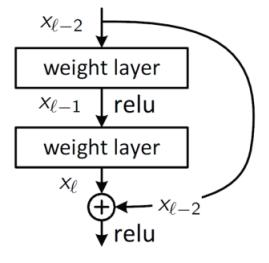
\includegraphics[keepaspectratio,
                     width=.3\paperwidth]{skip-connection.jpg}
  \end{center}
\end{frame}

\begin{frame}
  \begin{itemize}
    \item (главное) Получается увеличивать число слоев
    \item Приращения более устойчивы $\to$ лучше сходимость
  \end{itemize}

  \noindent\rule{8cm}{0.4pt}

  {\it Kaiming He, Xiangyu Zhang, Shaoqing Ren, Jian Sun.} Deep Residual Learning for Image Recognition. 2015.

  {\it R.K. Srivastava, K. Greff, J. Schmidhuber.} Highway Networks. 2015
\end{frame}


\begin{frame}
  \frametitle{ResNet: визуализация оптимизационного критерия}

\begin{center}
  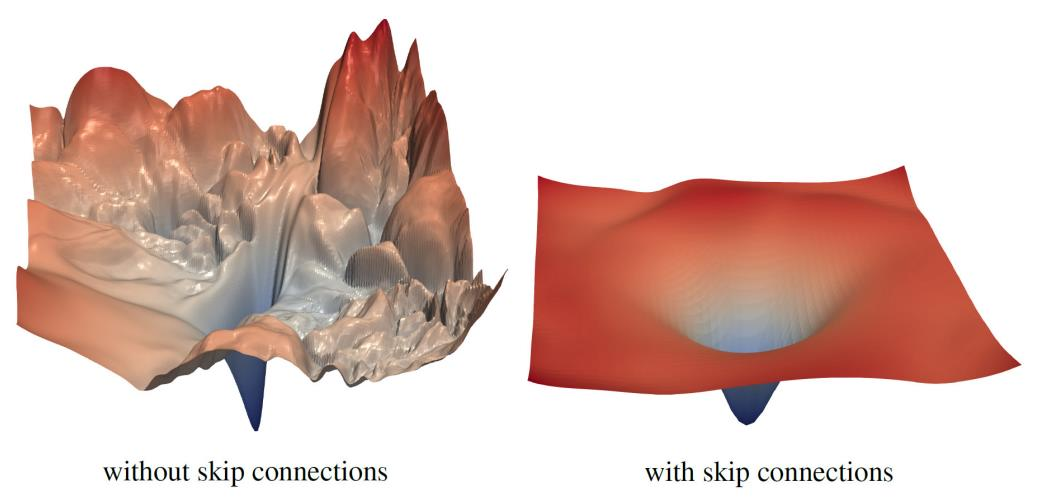
\includegraphics[keepaspectratio,
                   width=0.7\paperwidth]{skip-connection-opt.jpg}
\end{center}

  \noindent\rule{8cm}{0.4pt}

  {\it Hao Li et al.} Visualizing the Loss Landscape of Neural Nets. 2018.
\end{frame}


\begin{frame}
  \frametitle{WideResNet — WRN}
  Недостатки ResNet
  \begin{itemize}
    \item слишком глубокие — до 1000 слоев :)
    \item долго обучаются до SotA
  \end{itemize}

  \begin{center}
    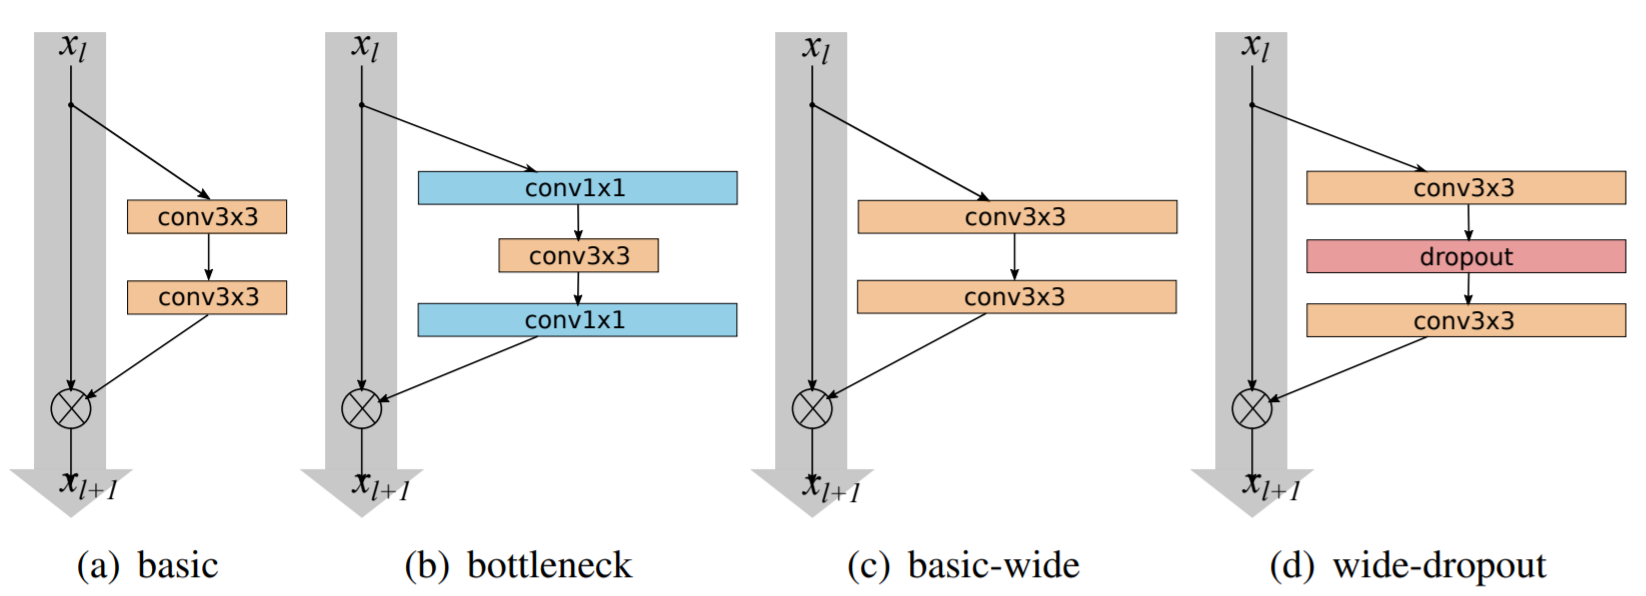
\includegraphics[keepaspectratio,
                     width=0.6\paperwidth]{wrn_blocks.png}
  \end{center}

  \begin{itemize}
    \item простая WRN сеть из 16 слоев победила все ResNet
    \item WRN-40-4 (т.е. 40 слоев и 4х ширина) обучается в 8 раз быстрее, чем ResNet-1001
  \end{itemize}

  \noindent\rule{8cm}{0.4pt}

  {\it S. Zagoruyko, N. Komodakis} \href{https://arxiv.org/pdf/1605.07146.pdf}{Wide Residual Networks, 2017}
\end{frame}


\begin{frame}
  \frametitle{Резюме}
  \begin{itemize}
    \item Свёрточные сети очень хорошо подходят для обработки изображений
    \item Различные алгоритмы оптимизации: adam, RMSProp
    \item Методы регуляризации: dropout, $L_2$ и batch normalization
    \item Ещё важен выбор начального приближения (инициализация весов)
    \item ResNet и skip-connections, WideResNet
  \end{itemize}

  \pause
  Что ещё можно посмотреть?
  \begin{itemize}
    \item Лекция курса в Стенфорде \href{https://www.youtube.com/watch?v=DAOcjicFr1Y}{о свёрточных сетях}
    \item Лекция К.В. Воронцова \href{https://youtu.be/Wwv-orQPMDg}{<<Нейронные сети: градиентные методы оптимизации>>}
  \end{itemize}
\end{frame}

\end{document}
